% ============================================================
%  DLCO 实验报告模板（lab01 实例）
%  【复用】复制整个 report/ 到 labNN/report/，改 \expname、\expdate + TODO 处 + 换 figures/ 图片
%  【编译】整个 lab 目录上传 tex.nju.edu.cn，编译 main.tex，下载 main.pdf 放回本目录
%  【提交】工程文件 + 报告电子版打包 zip 上传
% ============================================================
\documentclass[12pt, a4paper]{ctexart}

\usepackage{geometry}
\geometry{left=2.5cm, right=2.5cm, top=3cm, bottom=3cm}
\usepackage{listings}
\usepackage{graphicx}
\usepackage{xcolor}
\usepackage{amsmath}
\usepackage{tikz}

\graphicspath{{figures/}}

% ---------------- 代码高亮设置 ----------------
\lstset{
    language=Verilog,
    basicstyle=\ttfamily\small,
    frame=single,
    framesep=5pt,
    numbers=left,
    numberstyle=\tiny\color{gray},
    keywordstyle=\color{blue},
    commentstyle=\color{gray},
    breaklines=true,
    showstringspaces=false,
    tabsize=4
}

% ---------------- 封面信息（复用改 \expname、\expdate） ----------------
\newcommand{\coursename}{数字逻辑与计算机组成实验}
\newcommand{\expname}{lab01：选择器与优先编码器}   % TODO 改实验名
\newcommand{\expdate}{2026-09-01}                 % TODO 改实验日期
\newcommand{\stuname}{法童}
\newcommand{\stuid}{251250046}
\newcommand{\stumail}{251250046@smail.nju.edu.cn}

\begin{document}

% 封面
\begin{titlepage}
    \centering
    \vspace*{4cm}
    {\Huge\bfseries 实验报告\par}
    \vspace{1.5cm}
    {\Large \coursename\par}
    \vspace{0.8cm}
    {\Large \expname\par}
    \vspace{3cm}
    {\large
    \begin{tabular}{rl}
        姓名： & \stuname \\
        学号： & \stuid \\
        邮箱： & \stumail \\
        实验时间： & \expdate \\
    \end{tabular}\par}
\end{titlepage}

\section{实验目的}
\begin{enumerate}
    \item 掌握二位四选一选择器的设计与实现，熟练使用 \texttt{always}/\texttt{case} 语句进行行为级描述。
    \item 掌握带使能端 8-3 优先编码器的设计与实现，使用 \texttt{casez} 处理优先编码，并结合七段数码管完成译码显示。
    \item 熟悉 FPGA 开发板拨码开关、LED、七段数码管的硬件映射与控制。
\end{enumerate}

\section{实验原理}
多路选择器从多路数据输入中，根据选择控制信号选出其中一路送到输出。优先编码器对输入的多位信号按优先级判断，输出最高优先级有效位对应的编码值。本次实验的两个电路均为纯组合逻辑电路，无需时钟、无内部记忆，输出随输入即时变化。

\section{实验环境与器材}
\begin{itemize}
    \item 开发板：Nexys A7-100T（FPGA 型号 xc7a100tcsg324-1）
    \item 开发工具：Vivado 2020.2
    \item 硬件描述语言：Verilog HDL
\end{itemize}

\section{设计思路}

\subsection{选择器（exp1）}
模块含四个 2 位数据输入 $X_0\sim X_3$ 和一个 2 位选择控制输入 $Y$，利用 \texttt{case} 语句实现 4 选 1，将 $Y$ 指定的那路数据输出到 $F$。原理框图如下：

\begin{figure}[htbp]
    \centering
    \begin{tikzpicture}[every node/.style={font=\small}]
        \node[draw, minimum width=2.4cm, minimum height=2.4cm, align=center] (mux) at (0,0) {4 选 1\\选择器};
        \node[anchor=east] (x0) at (-2.4,1.4) {$X_0$[1:0]};
        \node[anchor=east] (x1) at (-2.4,0.45) {$X_1$[1:0]};
        \node[anchor=east] (x2) at (-2.4,-0.45) {$X_2$[1:0]};
        \node[anchor=east] (x3) at (-2.4,-1.4) {$X_3$[1:0]};
        \node[anchor=north] (y) at (0,-2.1) {$Y$[1:0]（选择）};
        \node[anchor=west] (f) at (2.4,0) {$F$[1:0]};
        \draw[->] (x0) -- (mux);
        \draw[->] (x1) -- (mux);
        \draw[->] (x2) -- (mux);
        \draw[->] (x3) -- (mux);
        \draw[->] (y) -- (mux);
        \draw[->] (mux) -- (f);
    \end{tikzpicture}
    \caption{选择器原理框图}
\end{figure}

核心逻辑（\texttt{case} 语句）：
\begin{lstlisting}
always @(*)
    case (Y)
        0: F = X0;
        1: F = X1;
        2: F = X2;
        3: F = X3;
    endcase
\end{lstlisting}

\subsection{优先编码器（exp2）}
实现带使能端的高位优先 8-3 编码器：用 \texttt{casez} 做含通配符的模式匹配，使能有效时输出最高位 1 对应的编码值及有效标志；编码值再经 \texttt{bcd7seg} 模块译成七段数码管段选。原理框图如下：

\begin{figure}[htbp]
    \centering
    \begin{tikzpicture}[every node/.style={font=\small}]
        \node[anchor=east] (x) at (-4.2,0.6) {$X$[7:0]};
        \node[anchor=east] (en) at (-4.2,-0.6) {$en$};
        \node[draw, minimum width=2.2cm, minimum height=1.8cm, align=center] (enc) at (-0.4,0) {8-3 优先\\编码器};
        \node[draw, minimum width=1.8cm, minimum height=1.6cm, align=center] (seg) at (2.6,0) {bcd7seg\\译码};
        \node[anchor=west] (segout) at (4.8,0) {段选 CA$\sim$CG};
        \node[anchor=north] (zv) at (0.6,-1.9) {$Z$[2:0]、$valid$};
        \draw[->] (x) -- (enc);
        \draw[->] (en) -- (enc);
        \draw[->] (enc) -- (seg);
        \draw[->] (seg) -- (segout);
        \draw[->] (enc) -- (zv);
    \end{tikzpicture}
    \caption{优先编码器原理框图}
\end{figure}

核心逻辑（\texttt{casez} 语句）：
\begin{lstlisting}
casez (X)
    8'b1???????: begin Y = 4'b0111; valid = 1'b1; end
    8'b01??????: begin Y = 4'b0110; valid = 1'b1; end
    8'b001?????: begin Y = 4'b0101; valid = 1'b1; end
    ...  // 依次类推，直至 8'b00000001
    default:    begin Y = 4'b1111; valid = 1'b0; end
endcase
\end{lstlisting}

\section{实验过程}
\begin{enumerate}
    \item 编写功能模块：分别实现选择器 \texttt{exp1} 与优先编码器 \texttt{exp2} 的逻辑模块，再按 \texttt{top} 包装模式编写顶层模块，把逻辑端口与板级引脚（\texttt{SW}、\texttt{LED}、七段数码管）相连。
    \item 编写约束文件：从根目录的 \texttt{nexysa7.xdc} 复制，仅取消本次实验用到引脚的注释（注意 \texttt{SW[8]} 为 LVCMOS18），生成 \texttt{exp1.xdc} / \texttt{exp2.xdc}。
    \item 综合与实现：运行 \texttt{build.bat} 完成综合、布局布线，生成比特流 \texttt{build/top.bit}。
    \item 下载运行：运行 \texttt{prog.bat} 将比特流下载到开发板，拨动开关观察 LED / 数码管输出。
\end{enumerate}

% TODO：适当截图展示重要步骤（如 Vivado 综合/实现完成、下载成功），取消下面注释
% \begin{figure}[htbp]
%     \centering
%     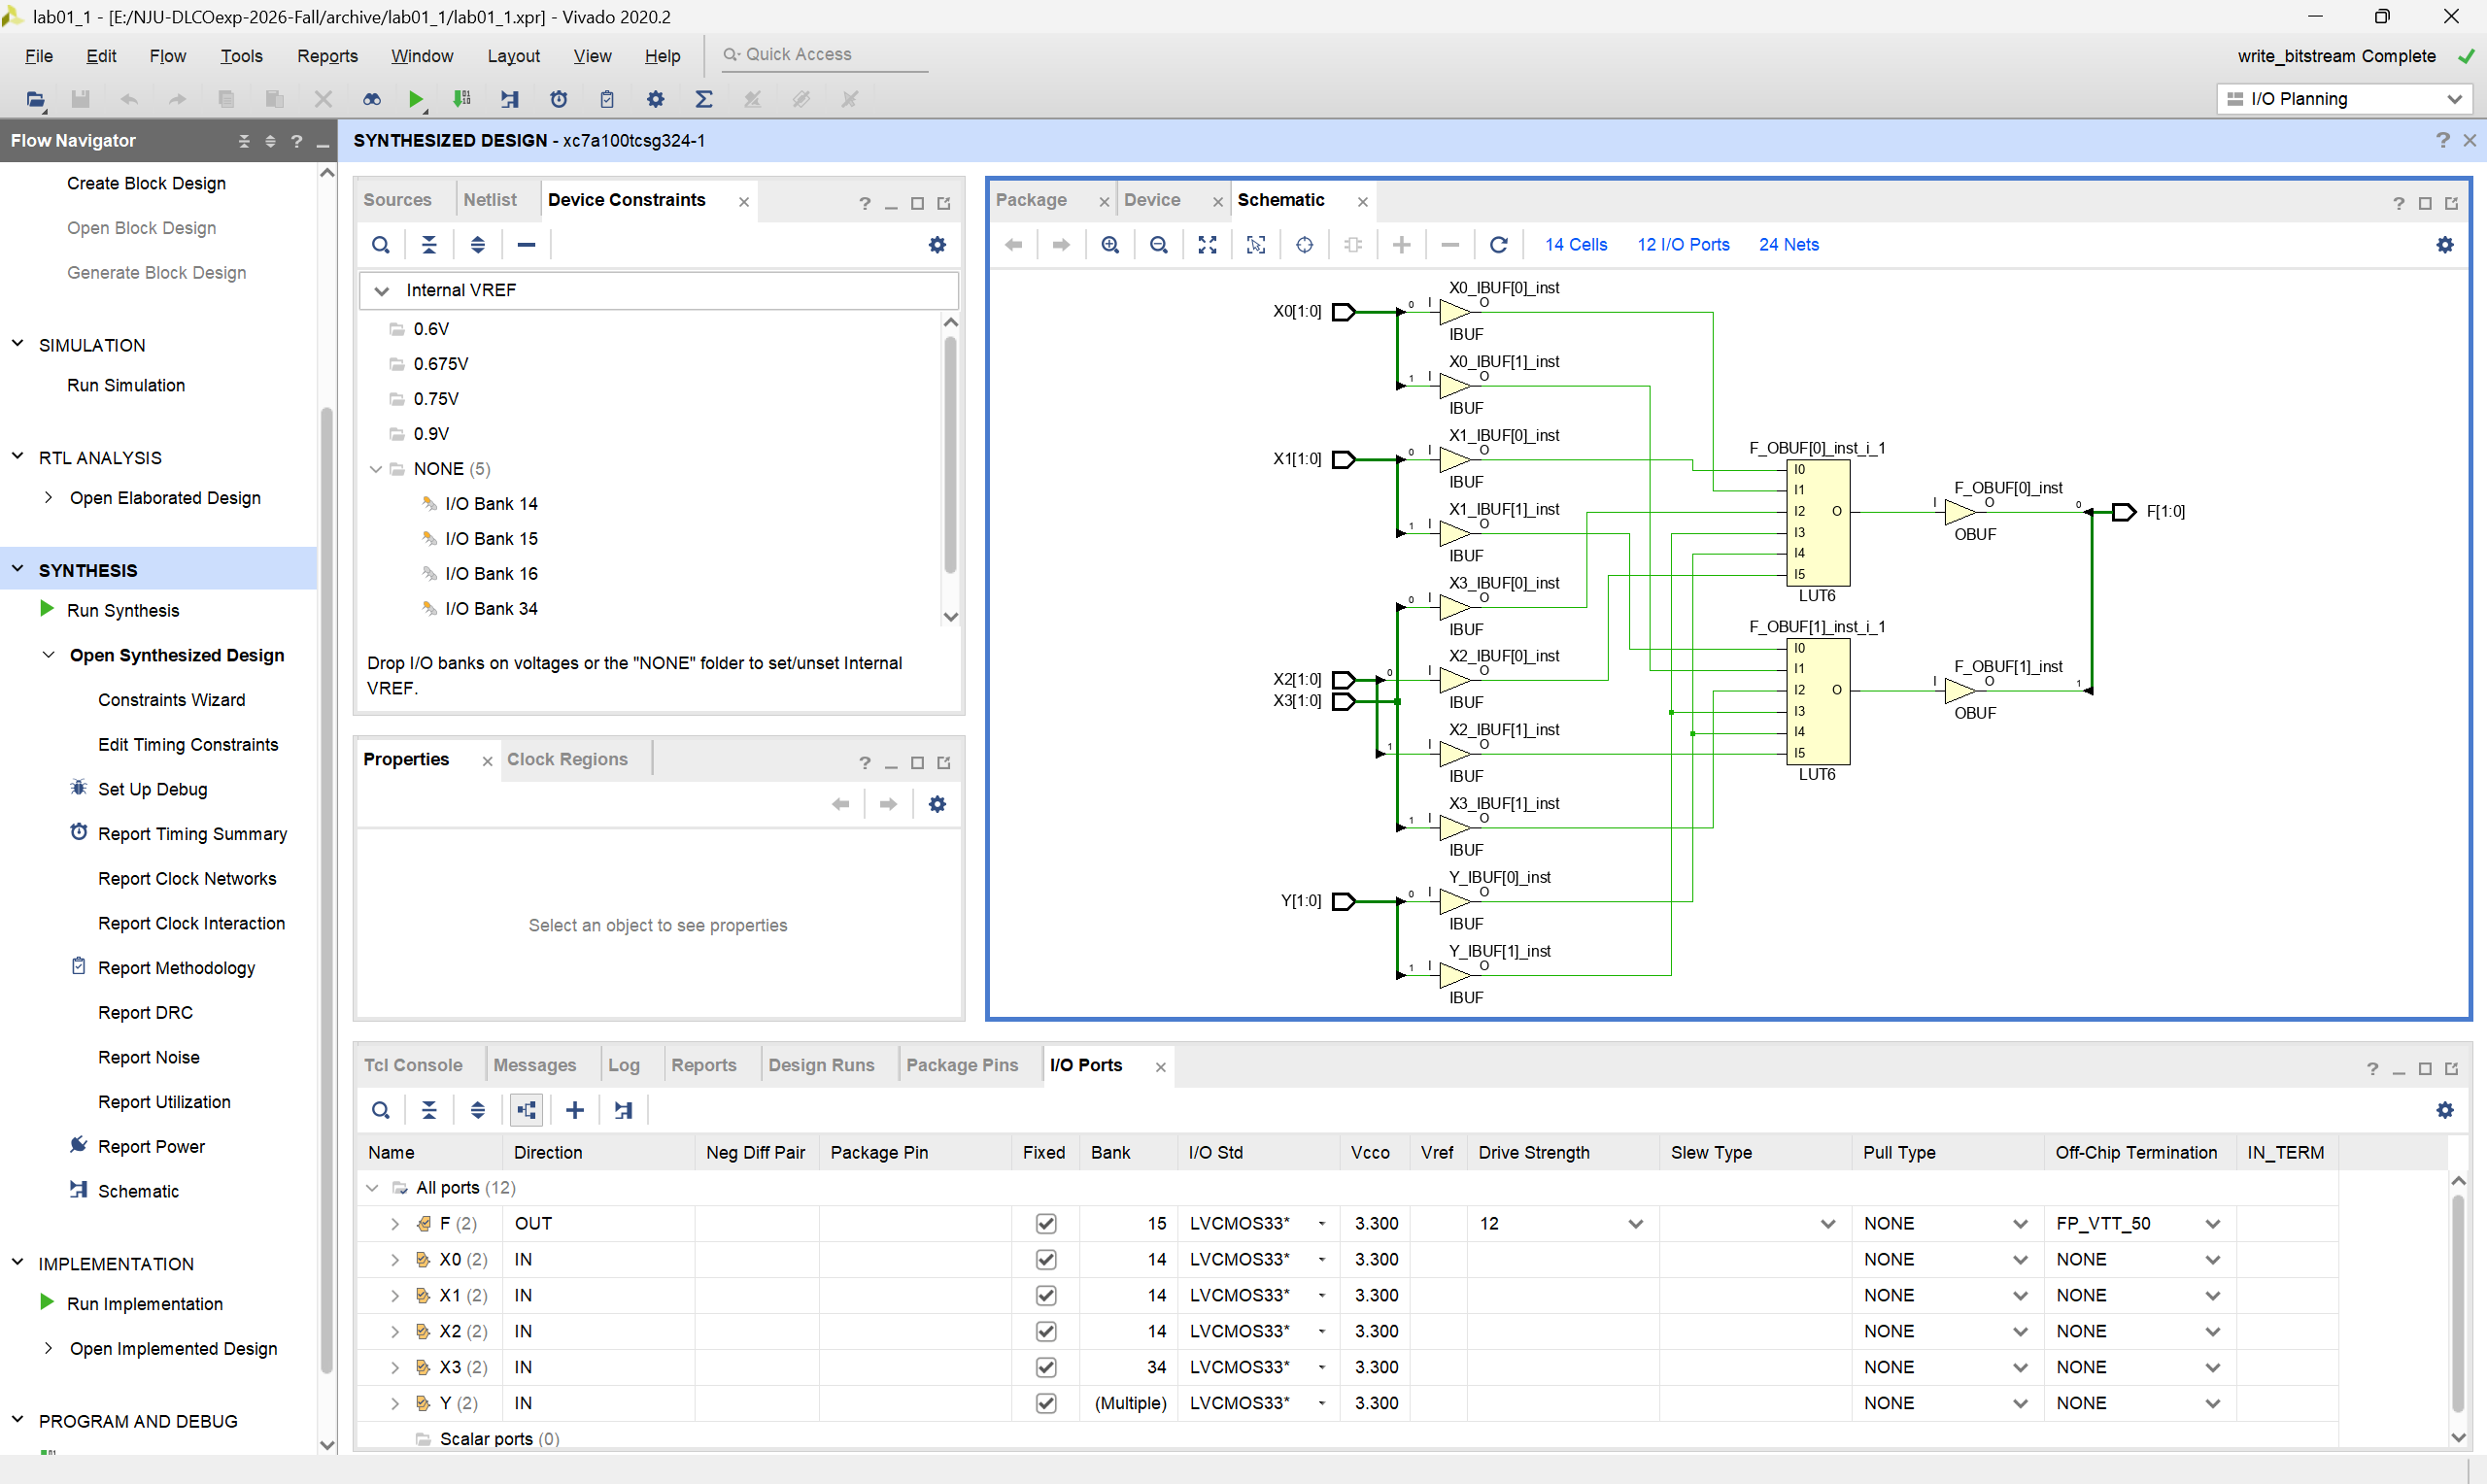
\includegraphics[width=0.7\textwidth]{exp1_build.png}
%     \caption{Vivado 综合与实现完成}
% \end{figure}

\section{测试方法}
验证方法上，本实验从两方面确认设计正确性：一是用 Vivado 做功能仿真、观察波形图验证逻辑正确，二是下载到开发板实测。测试信号的选择上，选择器遍历选择端 $Y$ 的 00/01/10/11，并给四个输入 $X_0\sim X_3$ 赋不同特征值，验证 4 选 1 逻辑；优先编码器用单个 1 依次测试各优先级别、用多个 1 测试优先级覆盖、用全 0 和未使能测试边界情况。

\section{实验结果}

\subsection{选择器（exp1）}
% TODO：贴 Vivado 仿真波形截图，取消下面注释（图片命名如 exp1_wave.png 放 figures/）
% \begin{figure}[htbp]
%     \centering
%     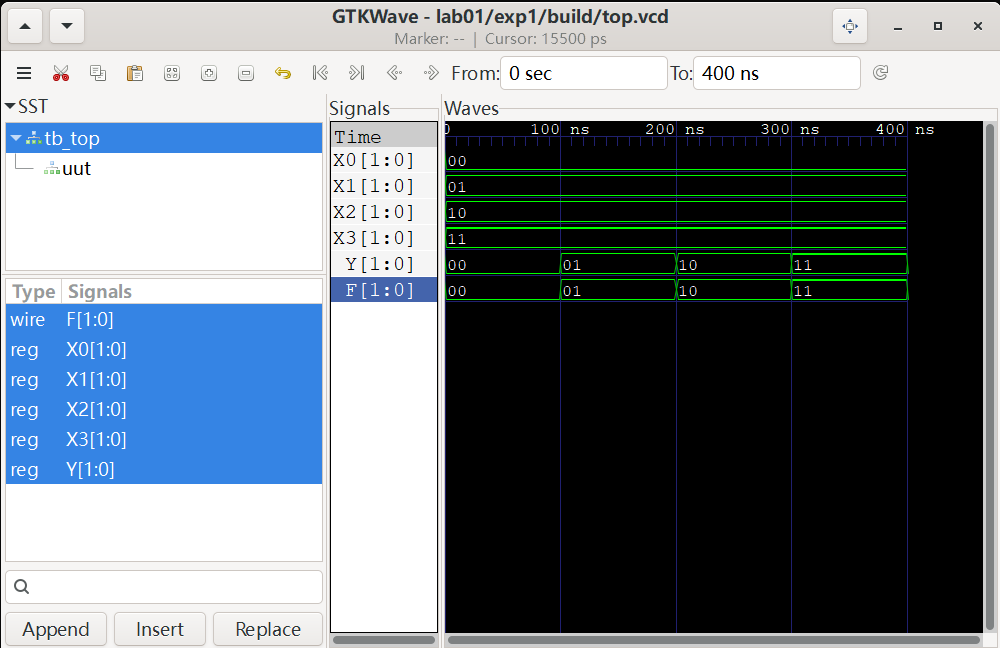
\includegraphics[width=0.7\textwidth]{exp1_wave.png}
%     \caption{选择器仿真波形}
% \end{figure}
% TODO：贴上板运行结果，取消下面注释（图片命名如 exp1_board.jpg 放 figures/）
% \begin{figure}[htbp]
%     \centering
%     \includegraphics[width=0.6\textwidth]{exp1_board.jpg}
%     \caption{选择器上板运行结果}
% \end{figure}
（现象描述：拨动 \texttt{SW[1:0]} 选择开关，\texttt{LED[1:0]} 输出对应的 $X_0\sim X_3$ 数据，验证 4 选 1 功能。）

\subsection{优先编码器（exp2）}
% TODO：贴 Vivado 仿真波形截图，取消下面注释（图片命名如 exp2_wave.png 放 figures/）
% \begin{figure}[htbp]
%     \centering
%     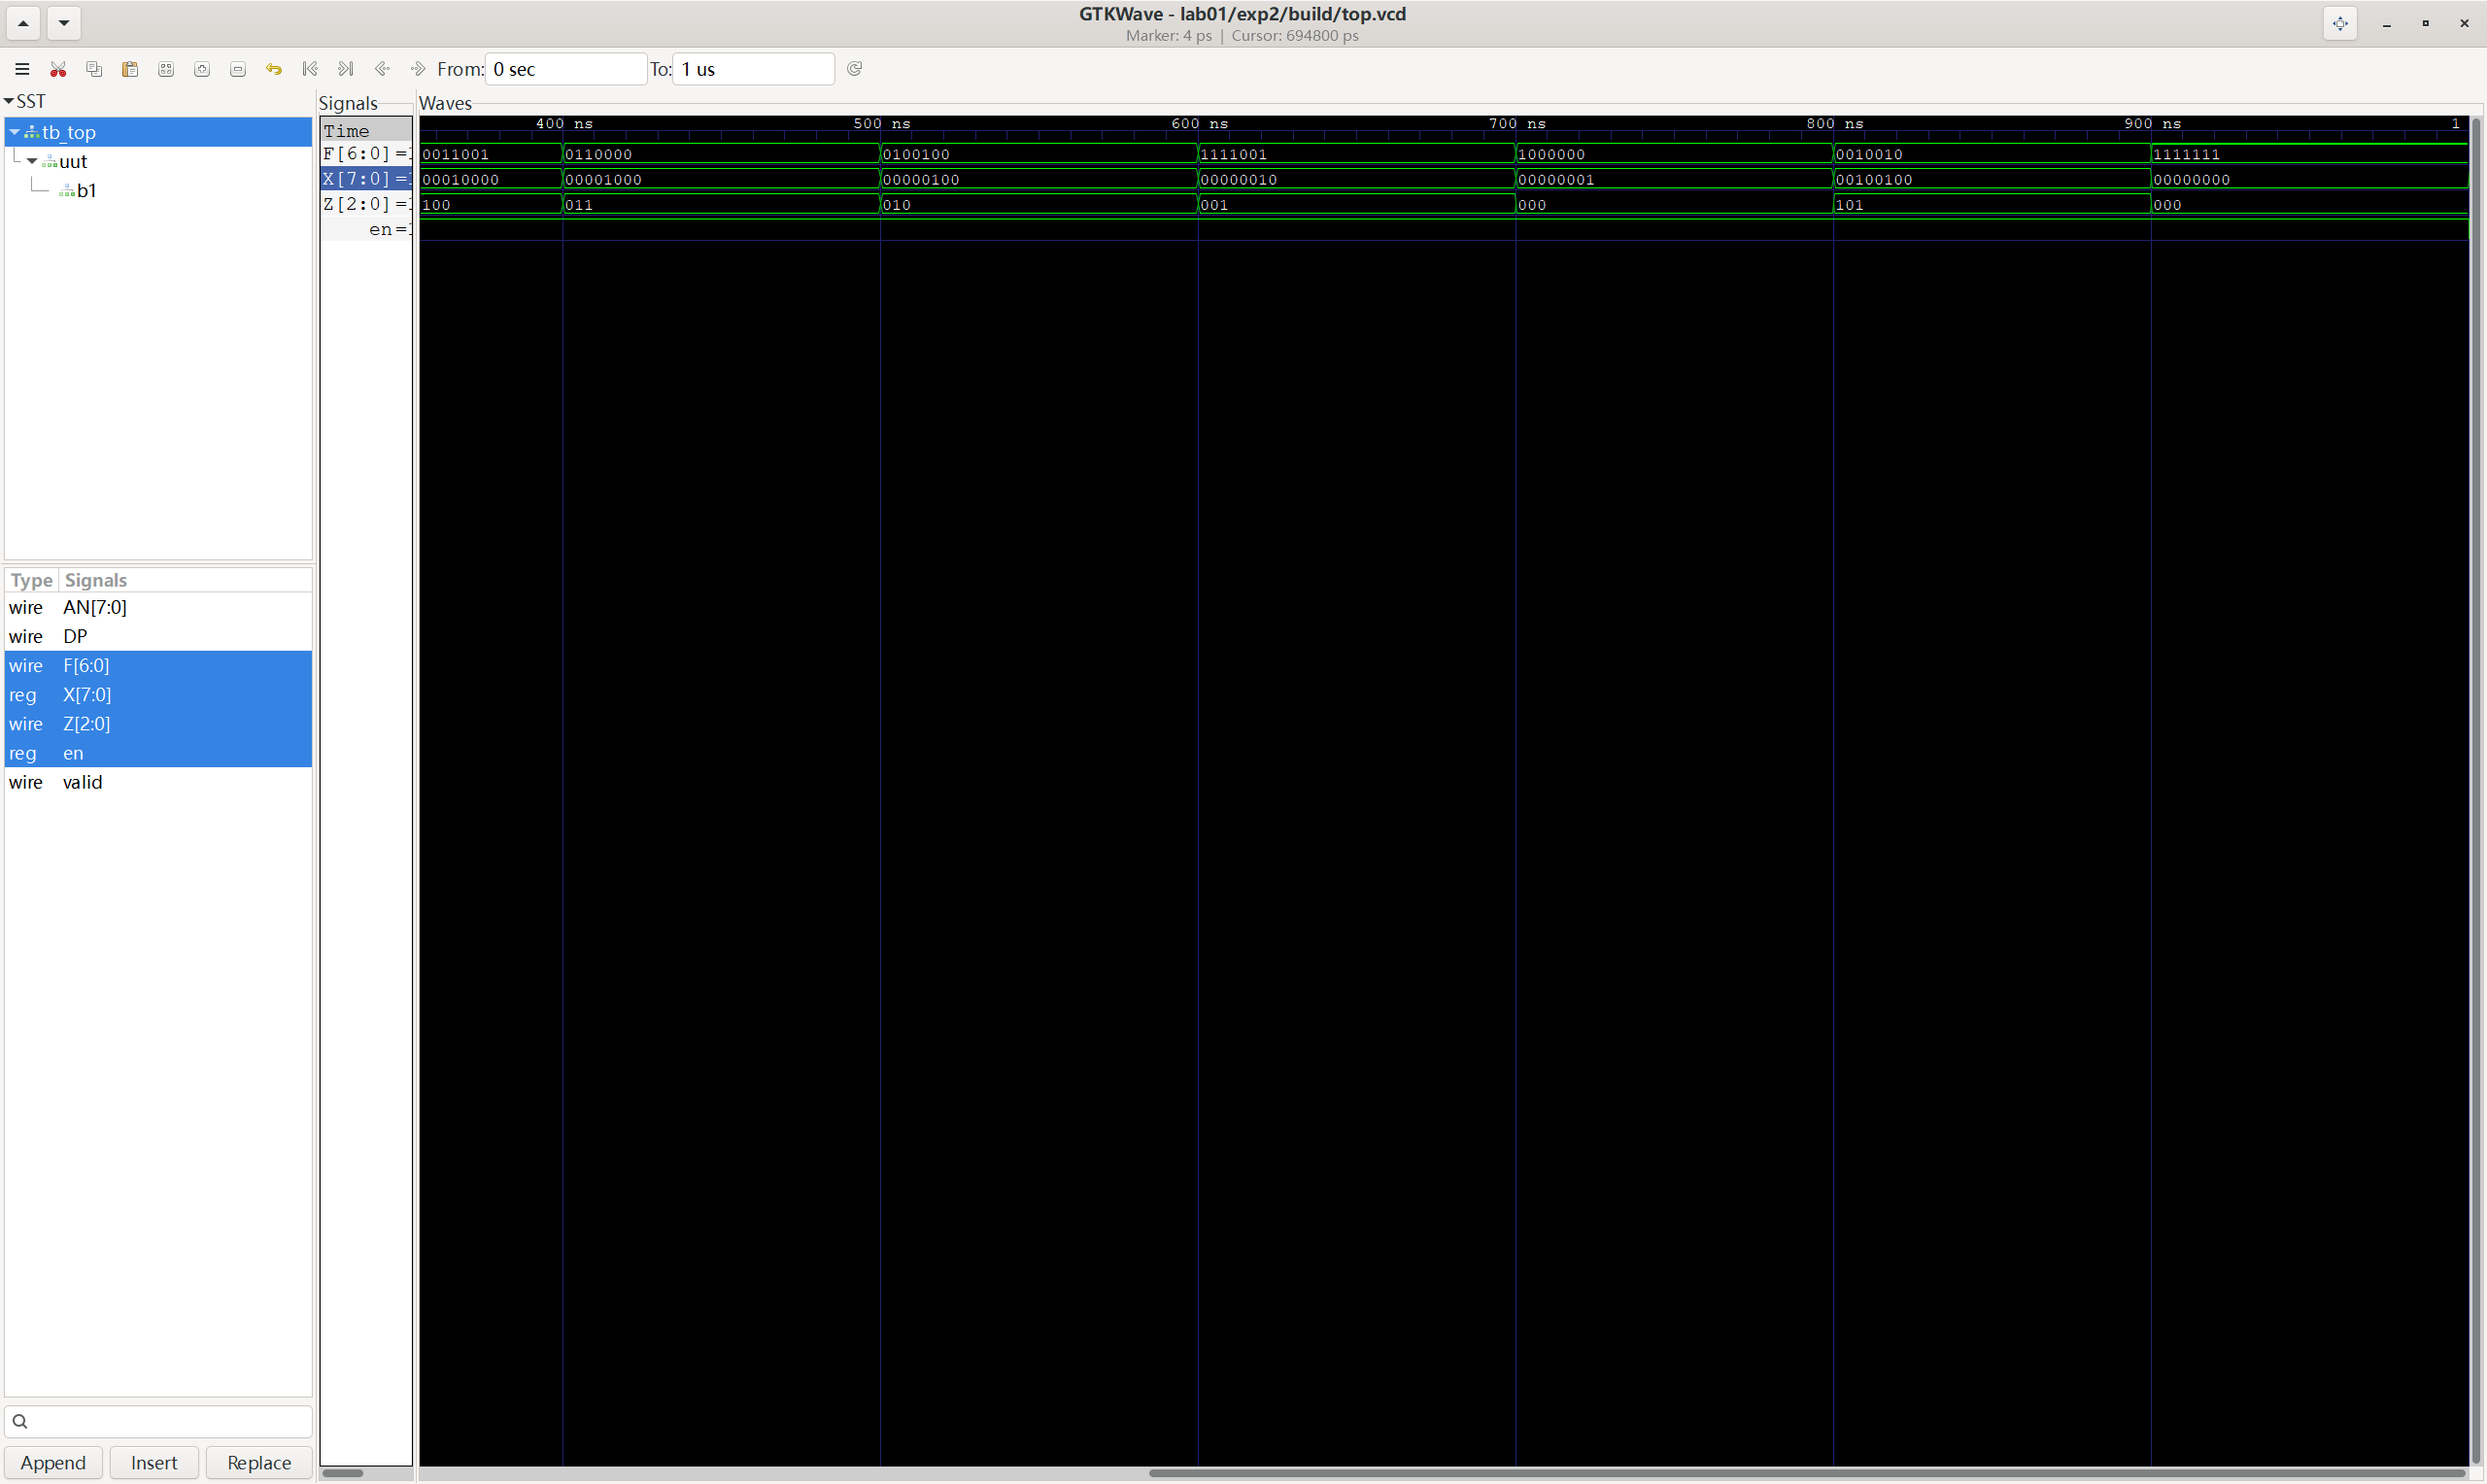
\includegraphics[width=0.7\textwidth]{exp2_wave.png}
%     \caption{优先编码器仿真波形}
% \end{figure}
% TODO：贴上板运行结果，取消下面注释（图片命名如 exp2_board.jpg 放 figures/）
% \begin{figure}[htbp]
%     \centering
%     \includegraphics[width=0.6\textwidth]{exp2_board.jpg}
%     \caption{优先编码器上板运行结果}
% \end{figure}
（现象描述：使能 \texttt{SW[8]} 后拨动 \texttt{SW[7:0]}，数码管与 \texttt{LED} 显示最高位 1 对应的编码值。）

\section{问题与解决办法}
\begin{itemize}
    \item \textbf{未使用位未约束导致报错}：exp2 中输出 \texttt{LED[3]} 未使用，但未约束触发布局布线警告/错误。解决：在 \texttt{top.v} 中将其置 0，并在 \texttt{.xdc} 中补上约束。
    \item \textbf{数码管多位同时点亮/小数点误亮}：exp2 只用一位数码管显示编码值，最初未处理位选与小数点，导致多位数码管同时点亮、小数点误亮。原因：Nexys A7 的位选 \texttt{AN} 与段选、小数点均为低有效，需要选通最右一位并把小数点熄灭。解决：在模块内 \texttt{assign AN = 8'b11111110} 只拉低 \texttt{AN[0]}，并 \texttt{assign DP = 1'b1}。
\end{itemize}

\section{启示与建议}

\textbf{启示：}
\begin{enumerate}
    \item 初步掌握了 Verilog 的语法，如 \texttt{module}/\texttt{endmodule} 与端口声明、\texttt{wire}/\texttt{reg} 数据类型、\texttt{assign} 连续赋值、\texttt{always @(*)} 组合逻辑、\texttt{case}/\texttt{casez} 语句以及总线拼接 \texttt{\{\}} 等。
    \item 掌握了通过 Verilog HDL 描述组合逻辑电路，并完成仿真、综合、上板测试的完整操作流程。
    \item 发现了 \texttt{top.v} 顶层模块结合 \texttt{.xdc} 缺省源配置接口约束的便利性。
\end{enumerate}

\textbf{建议：} 建议把 \texttt{top.v} 顶层模块结合 \texttt{.xdc} 缺省源配置接口约束的便捷方法推广到课程教学中，帮助学生更有效率、更有条理地完成实验。

\end{document}
